% Created 2019-01-22 Di 08:26
% Intended LaTeX compiler: pdflatex
\documentclass[10pt, a4paper]{scrartcl}
\usepackage[utf8]{inputenc}
\usepackage[T1]{fontenc}
\usepackage{graphicx}
\usepackage{grffile}
\usepackage{longtable}
\usepackage{wrapfig}
\usepackage{rotating}
\usepackage[normalem]{ulem}
\usepackage{amsmath}
\usepackage{textcomp}
\usepackage{amssymb}
\usepackage{capt-of}
\usepackage{hyperref}
\usepackage[ngerman, germanb]{babel}
\usepackage[a4paper,margin=2.54cm]{geometry}
\date{2018-07-23 17:52}
\title{Bereinigung von mehrfach-Holdings}
\hypersetup{
 pdfauthor={Stefan Schuh},
 pdftitle={Bereinigung von mehrfach-Holdings},
 pdfkeywords={},
 pdfsubject={},
 pdfcreator={Emacs 25.2.2 (Org mode 9.2)}, 
 pdflang={Germanb}}
\begin{document}

\maketitle
\tableofcontents



\section{Ausgangslage und Ziel}
\label{sec:org6604db8}
Bei der Datenvorbereitung vor der Migration konnten nicht alle Exemplare einem
Holding zugeordnet werden, weil in Aleph kein HOL vorhanden war. Infolgedessen
gibt es Titeldatensätze mit bis zu 678 Holdings mit je einem Item.

\href{data/DHB\_ITEMS\_ohne\_HOL\_20180717.xlsx}{Auswertung (Aleph) der DHB-Datensätze ohne Holding}

Es handelt sich um insgesamt 41639 Exemplare an 291 AC-Sätzen und 2394 LB-Sätzen.

Ziel ist es, die Exemplare an diesen mehrfach-HOLs an ein einzelnes Holding zu
hängen und die überschüssigen HOLs zu löschen. Dies sollte in einem
halbautomatischen Prozess passieren (wenn es vollautomatisch ginge, hätten wir
das wohl schon vorher in Aleph gemacht), weil eine manuelle Bereinigung nicht
leistbar ist.

\subsection{Angestrebter Workflow}
\label{sec:orgdf683e4}
Eine Bearbeiterin stößt auf einen der betroffenen Datensätze und will ihn
bereinigen. Dazu sollte sie die folgenden Schritte ausführen müssen:

\begin{enumerate}
\item Das Holding anlegen, an dem die Items im Endeffekt hängen sollen. Wichtig
ist, dass zumindest Bibliothek, Standort und Grundsignatur eingetragen
werden, weil über diese ein Abgleich stattfindet. Wenn notwendig mehrere
HOLs (für Indexe, neue folgen, etc.).
\item Das Bereinigungsprogramm aufrufen und folgende Daten eingeben:
\begin{itemize}
\item MMS-ID des Titeldatensatzes (*3339)
\item MMS-ID des Zielholdings
\end{itemize}
\end{enumerate}


\subsection{Was soll das Script leisten?}
\label{sec:org64e7b7e}
Im Endeffekt sollen alle Items an ihren richtigen Holdings hängen. Dazu
sollte aus dem Zielholdings die Grundsignatur ausgelesen werden. Nur
Exemplare, bei denen Bibliothek, Standort und Grundsignatur mit dem Holding
übereinstimmen, sollten an das jeweilige Holding gehängt werden.


\subsubsection{Mögliche Probleme}
\label{sec:org03a6b5a}
\begin{itemize}
\item Für die Bearbeiterin
\begin{itemize}
\item Bei großen Anzahlen an Holdings ist es nicht leicht feststellbar, ob
mehrere Zielholdings (für neue Folgen, Indizes etc.) angelegt werden
müssen.
\end{itemize}
\item Für das Programm
\begin{itemize}
\item Sind Bestellungen mit einem der vorhandenen HOLs verknüpft?
\item Verschiedene Grundsignaturen können mit demselben String anfangen: \texttt{I
          123/1} und \texttt{I 123/N.F.,1}
\end{itemize}
\end{itemize}

\section{Skript}
\label{sec:orga97f21d}

\subsection{Allgemeine Vorbereitungen}
\label{sec:org91ee690}
Dieses Script benötigt Python 3.6 oder höher.
\subsubsection{Python Virtual environment}
\label{sec:orged6d5e4}
Damit immer die richtigen Versionen des Interpreters und der Module
verwendet werden, erstellen wir eine Virtual Environment. Dazu führen wir
in der Shell folgendes aus:

\begin{verbatim}
# Die virtuelle Umgebung erstellen
python -m venv ~/.venvs/multi-hol

# Die virtuelle Umgebung aktivieren
source ~/.venvs/multi-hol/bin/activate
\end{verbatim}


\subsubsection{Imports etc.}
\label{sec:org3c112c6}
Als erstes importieren wir verschiedenen Module, die wir brauchen:

\begin{verbatim}
import sys
import re
import os
import keyring
import datetime
from requests import Session
import urllib.parse
import xml.etree.ElementTree as ET
import json
from time import sleep
from easygui import multenterbox
import logging
import getpass
\end{verbatim}

\begin{description}
\item[{\texttt{sys}}] um Kommandozeilenargumente entgegenzunehmen (\texttt{sys.argv}) oder
die Ausführung abzubrechen (\texttt{sys.exit})
\item[{\texttt{os}}] Verzeichnisse anlegen, Dateien löschen, etc.
\item[{\texttt{keyring}}] dient dazu, den API-Key aus dem System-Keyring zu lesen. Für die
Distribution ist das natürlich nicht brauchbar. Im Endeffekt wird man hier
den Key wohl direkt reinschreiben müssen. Achtung: Dieses
Modul gehört nicht zur Standardbibliothek und muss erst via
\texttt{pip} installiert werden.
\item[{\texttt{requests.Session}}] vereinfacht die API-Calls, indem man die Header
nicht immer eingeben muss, etc. Achtung: Dieses Modul gehört
nicht zur Standardbibliothek und muss erst via \texttt{pip} installiert
werden.
\item[{\texttt{urllib.parse}}] wird verwendet, um Strings, die als Teil des URL
verwendet werden, richtig zu codieren
\item[{\texttt{xml.etree.ElementTree}}] Nachdem wir nicht viel brauchen, ist es
einfacher XML zu parsen als die Holdings in pymarc zu lesen, oder in
JSON umzuwandeln.
\item[{\texttt{json}}] Wir bekommen von der Alma Item-Objekte als JSON. Mit dieser Bibliothek
lassen sich JSON-Daten gut manipulieren.
\item[{\texttt{time.sleep}}] um zwischen Löschen am Quell- und Posten am Zielholding
zu warten
\item[{\texttt{easygui.multenterbox}}] um von der Benutzerin die MMS-ID von Bibsatz
und Zielholding zu bekommen
\item[{\texttt{logging}}] um zu loggen
\item[{\texttt{getpass}}] damit wir fürs loggen den Usernamen abfragen können
\end{description}

\subsubsection{{\bfseries\sffamily DONE} Logging}
\label{sec:orgaf2d57e}
Falls etwas danebengeht, wollen wir genau wissen, was passiert ist. Daher
loggen wir alles mit, was passiert. Fast alles -- nachdem wir für den
Dateinamen die MMS-IDs brauchen holen wir uns selbige schon, bevor wir den
logger konfigurieren (\ref{org13bdfcd}).

\begin{verbatim}
# now = datetime.datetime.now().strftime("%Y%m%d%H%M%S")
log_file = os.path.join(backup_dir, f"{bib_mms}_{target_hol_id}.log")
logger = logging.getLogger(__name__)
logger.setLevel(logging.DEBUG)
logger.propagate = False

# add handlers
log_stream_handler = logging.StreamHandler(sys.stdout)
log_stream_handler.setLevel(logging.INFO)
log_stream_handler.setFormatter(
    logging.Formatter('%(levelname)s: %(message)s'))
logger.addHandler(log_stream_handler)

log_file_handler = logging.FileHandler(log_file)
log_file_handler.setLevel(logging.DEBUG)
log_file_handler.setFormatter(
    logging.Formatter('%(asctime)s - %(levelname)s - %(message)s'))
logger.addHandler(log_file_handler)

# tell us who started the program
logger.debug(f"Programm gestartet von {getpass.getuser()}.")
\end{verbatim}

\subsubsection{Voreinstellungen für die APIs}
\label{sec:org94cf360}
Nachdem wir viele Calls machen werden, ist es wohl gut, die APIs in
Variablen mit benannten Platzhaltern zu schreiben, sodass wir dann nur
noch die jeweiligen IDs einfüllen müssen:

\begin{verbatim}
# api-url-templates
base_url = 'https://api-eu.hosted.exlibrisgroup.com/almaws/v1'
barcode_api = base_url + "/items?item_barcode={barcode}"
holdings_api = base_url + "/bibs/{mms_id}/holdings"
bib_api = base_url + "/bibs/{mms_id}"
item_api = base_url + "/bibs/{mms_id}/holdings/{holding_id}/items"
\end{verbatim}

\subsubsection{Session, Authentifizierung}
\label{sec:org5749621}
Damit wir nicht bei jedem Aufruf die Header übergeben müssen, ist es
praktisch, dass die requests-Bibliothek ein Session-Objekt hat.

\begin{verbatim}
# session um immer gleiche header zu schicken etc.
session = Session()
session.headers.update({
    "accept": "application/json",
    "authorization": f"apikey {api_key}"
})
\end{verbatim}

Den API-Key hole ich mit der keyring-Bibliothek aus dem System-Keyring.
Für eine Deployment-Version muss man den Key wohl hereinschreiben.

\begin{verbatim}
# get api key from system keyring
api_key = keyring.get_password("ALMA-API", "BIB-Sandbox").rstrip()
\end{verbatim}

\subsection{Verarbeitung}
\label{sec:orgce2d7d8}
\subsubsection{{\bfseries\sffamily DONE} Feststellen, welche Datensätze bearbeitet werden sollen und ein paar Daten auslesen}
\label{sec:org434b757}
Um zu wissen, an welchen Datensätzen gearbeitet werden soll, muss die
Bearbeiterin die MMS-IDs vom Bibsatz und dem Zielolding eingeben.

Nachdem Whitespace vorne und hinten entfern wurde, sollte folgendes
überprüft werden:
\begin{itemize}
\item[{$\boxtimes$}] Beginnt die bib-mms mit 99?
\item[{$\boxtimes$}] Beginnt die hol-mms mit 22?
\item[{$\boxtimes$}] Endet die bib-mms auf 3339?
\end{itemize}
\begin{verbatim}
def get_mmsids(msg=""):
    """Return the MMS-IDs of the bibrecord and the target-holding."""

    if msg == "":
        msg =  "Bitte folgende Daten eingeben."
    else:
        msg = msg

    bib_mms, target_hol_id = multenterbox(msg=msg,
                                           title="Multi-HOL-Bereinigung",
                                           fields=["MMS-ID des Bibsatzes", "MMS-ID des Zielholdings"])
    # check the input
    if (not bib_mms.startswith("99")
            or not bib_mms.endswith("3339")
            or not target_hol_id.startswith("22")):
        msg = """*** Formaler Fehler in der Eingabe ***

    1. Die MMS-ID des Bibsatzes muss mit "99" beginnen
    2. Die MMS-ID des Bibsatzes muss mit "3339" enden
    3. Die MMS-ID des HOL-Satzes muss mit "22" beginnen
"""
        get_mmsids(msg)
    else:
        return bib_mms, target_hol_id

# assign values to bib_mms and target_hol_id
if len(sys.argv) == 3:
    bib_mms = sys.argv[1]
    target_hol_id = sys.argv[2]
else:
    bib_mms, target_hol_id = get_mmsids()
\end{verbatim}

\subsubsection{{\bfseries\sffamily DONE} Items holen}
\label{sec:orgf3379d2}
Nachdem die Bearbeiterin uns mit den Identifiern versorgt hat, holen wir
uns die Item-Liste. Nachdem die API per default nur zehn Items liefert,
setzen wir das Limit auf die höchstzahl (100). Sollten mehr als 100
Exemplare vorhanden sein, machen wir mehrere API-Aufrufe mit
entsprechendem Offset.

Dazu verwenden wir eine Funktion, die die MMS-IDs des Bibsatzes und eine
Liste von Item-Objekten zurückgibt.

\begin{verbatim}
def get_items(mms_id, target_hol_id):
    mms_id = mms_id
    outlist = []
    hol_bch = get_bch(target_hol_id)

    # get the item-list from Alma
    item_list = session.get(item_api.format(mms_id=mms_id, holding_id="ALL"),
                            params={"limit": "100"})

    # TODO check response
    if item_list.status_code == 200:
        item_list = item_list.json()
    else:
        logger.error(f"Fehler beim Holen der Daten: {item_list.text}")
        input("Drücken Sie ENTER um das Programm zu beenden.")
        sys.exit(1)

    # append the items to the list to be returned, if they pass the tests
    logger.debug("get_items(): Items zur outlist hinzufügen")
    for item in item_list["item"]:
        if check_bch(item, hol_bch):
            outlist.append(item)

    # check if there are more than 100 items
    total_record_count = int(item_list["total_record_count"])
    if total_record_count > 100:
        # calculate number of needed additional calls
        add_calls = total_record_count // 100
        logger.debug(f"get_items(): {total_record_count} items vorhanden, {add_calls} weitere API-calls notwendig.")
        # make the additional calls and add answer to the outlist
        for i in range(add_calls):
            offset = (i + 1) * 100
            logger.debug(f"get_items(): additional call {offset}")

            next_list = session.get(item_api.format(mms_id=mms_id, holding_id="ALL"),
                                    params={"limit": "100", "offset": offset}).json()
            logger.debug(f"get_items(): weitere items zu outlist hinzufügen (call {offset}/{add_calls})")
            for item in next_list["item"]:
                if check_bch(item, hol_bch):
                    outlist.append(item)

    # DONE save the item list to disk
    logger.info("Schreibe Backup.")
    backup_file = os.path.join(backup_dir, f"{mms_id}_{hol_bch[0]}_{hol_bch[1]}_{hol_bch[2].replace('.', '').replace(',', '').replace('/', '').replace(' ', '-')}")
    save_json(outlist, backup_file)
    return outlist
\end{verbatim}

\subsubsection{{\bfseries\sffamily DONE} Inhaltliche Checks}
\label{sec:org2ce0e97}
Überprüfung, ob die richtigen Signaturen vorhanden sind, etc. Dazu holen
wir uns zuerst das Zielholding und lesen dort \texttt{856 b}, \texttt{c} und \texttt{h} aus.

\begin{verbatim}
def get_bch(holding_id):
    hol = session.get(holdings_api + "/" + holding_id, headers = {"accept": "application/xml"})
    try:
        holxml = ET.fromstring(hol.text)
        b = holxml.find('.//*[@tag="852"]/*[@code="b"]').text
        c = holxml.find('.//*[@tag="852"]/*[@code="c"]').text
        h = holxml.find('.//*[@tag="852"]/*[@code="h"]').text
    except:
        logger.exception("Fehler beim Lesen des Zielholdings (XML).")
        print("Ein Fehler ist aufgetreten. Kontrollieren Sie die Log-Datei.")
        input("Drücken Sie ENTER um das Programm zu beenden.")
        sys.exit(1)

    return b, c, h
\end{verbatim}

Dann schauen wir, ob das Item zum HOL passt, damit nicht
falschlicherweise Items von anderen Standorten oder mit anderen
Grundsignaturen umgehängt werden. Subfelder \texttt{b} und \texttt{c} müssen
übereinstimmen; die Signatur des Items (genaugenommen von dessen HOL)
muss mit demselben String anfangen, der in Subfeld \texttt{h} steht.

\begin{verbatim}
# check if the item fits the target holding's 852 b, c and h

def check_bch(item, hol_bch):
    """Check if the item fits the target holdings library, location and call number.

    Take an item object (dict) and return True or False."""

    hol_b, hol_c, hol_h = hol_bch

    item_b = item["item_data"]["library"]["value"]
    item_c = item["item_data"]["location"]["value"]
    item_h = item["holding_data"]["call_number"]
    item_alt = item["item_data"]["alternative_call_number"]
    item_h_from_alt = re.sub(r"^.* ; ", "", item_alt)

    bch_check = [False, False, False]

    if hol_b == item_b:
        bch_check[0] = True

    if hol_c == item_c:
        bch_check[1] = True

    if item_h.startswith(hol_h):
        bch_check[2] = True
    elif item_h_from_alt.startswith(hol_h):
        # if the item has already been moved to a false holding because the false
        # call number is a substring of the right one
        bch_check[2] = True

    if False in bch_check:
        return False
    else:
        return True
\end{verbatim}
\subsubsection{{\bfseries\sffamily DONE} Sicherungen machen}
\label{sec:org8d236e8}
\begin{enumerate}
\item {\bfseries\sffamily DONE} Das Sicherungsverzeichnis festlegen
\label{sec:org63b3563}
Hier legen wir das Verzeichnis fest, in das die Sicherungen und reports
kommen. Falls es nicht vorhanden ist, erstellen wir es.

\begin{verbatim}
backup_dir = os.path.join(os.path.expanduser("~"), "Dokumente", "ALMA_multi-hol")
# make the directory if it does not exist
if not os.path.exists(backup_dir):
    os.makedirs(backup_dir)
\end{verbatim}

\item {\bfseries\sffamily DONE} Items
\label{sec:org7c1219d}
Nachdem wir ja von \texttt{get\_items()} eine Liste mit Item-Objekten
zurückbekommen, schreiben wir diese einfach in eine Datei.

\begin{verbatim}
def save_json(json_list, filename, count=1):
    """Save JSON-file with a list of items to disk.

    Takes a list of JSON-objects."""

    fname = f"{filename}_{count}.json"
    try:
        with open(fname, "x") as backup:
            backup.write(json.dumps(json_list))
    except FileExistsError:
        save_json(json_list, filename, count + 1)
\end{verbatim}
\end{enumerate}

\subsubsection{{\bfseries\sffamily DONE} Änderungen an den Items machen}
\label{sec:orge72c9e0}
An den Exemplaren sind unter Umständen noch Änderungen vorzunehmen. Diese
beziehen sich in erste Linie auf die Signaturen.
\begin{enumerate}
\item {\bfseries\sffamily DONE} Bearbeitung der Signaturen
\label{sec:org2387f05}
Nachdem im Zielholding ja nur die Grundsignatur steht, würde diese
Information verloren gehen. Daher schreiben wir sie in die Alternative
Signatur des Exemplars.

Damit eine etwaig schon vorhandene alternative Signatur nicht
überschrieben wird, prüfen wir vorher, ob dort schon eine HB-Signatur
vorhanden ist. Wenn ja, wird die Signatur aus dem Holding nach \texttt{" ; "}
eingefügt.

\begin{verbatim}
alt_call_nr = item["item_data"]["alternative_call_number"]
hol_call_nr = item["holding_data"]["call_number"]

# check if the alternative call number is empty
if alt_call_nr == "":
    item["item_data"]["alternative_call_number"] = hol_call_nr
    item["item_data"]["alternative_call_number_type"]["value"] = 8
    item["item_data"]["alternative_call_number_type"]["desc"] = "Other scheme"
elif " ; " in alt_call_nr or hol_call_nr in alt_call_nr:
    pass
else:
    item["item_data"]["alternative_call_number"] = f"{alt_call_nr} ; {hol_call_nr}"

\end{verbatim}
\item {\bfseries\sffamily DONE} Exemplarstatus leeren
\label{sec:orgc41d725}
Wir nutzen diese Gelegenheit auch gleich, um den Exemplarstatus zu
löschen, der bei diesen Items in Alma nicht mehr notwendig ist.

\begin{verbatim}
item["item_data"]["policy"]["desc"] == None
item["item_data"]["policy"]["value"] == ''
\end{verbatim}

\item {\bfseries\sffamily DONE} Zusammensetzen der einzelnen Änderungen zu einer Funktion
\label{sec:org36d5015}
Damit die einzelnen Änderungen im Script ein bisschen übersichtlicher
zusammengefasst sind, ziehen wir sie in eine Funktion
\texttt{change\_item\_information()} zusammen, die wir dann während der
Bearbeitung aufrufen.

\begin{verbatim}
def change_item_information(item):
    """Make all necessary changes to the item object"""
    # Set the alternative call number
    alt_call_nr = item["item_data"]["alternative_call_number"]
    hol_call_nr = item["holding_data"]["call_number"]

    # check if the alternative call number is empty
    if alt_call_nr == "":
        item["item_data"]["alternative_call_number"] = hol_call_nr
        item["item_data"]["alternative_call_number_type"]["value"] = 8
        item["item_data"]["alternative_call_number_type"]["desc"] = "Other scheme"
    elif " ; " in alt_call_nr or hol_call_nr in alt_call_nr:
        pass
    else:
        item["item_data"]["alternative_call_number"] = f"{alt_call_nr} ; {hol_call_nr}"


    # clear the item policy
    item["item_data"]["policy"]["desc"] == None
    item["item_data"]["policy"]["value"] == ''
    return item
\end{verbatim}
\end{enumerate}
\subsubsection{{\bfseries\sffamily DONE} Items umhängen und Holdings löschen}
\label{sec:org3df8fc4}
Das Umhängen des Exemplars sollte der letzte Schritt sein. Vorher sollten
alle Checks laufen und das Item entsprechend angepasst werden (z. B. die
HOL-Signatur in die \texttt{alternative\_call\_number} schreiben).

Um ein Exemplar umzuhängen, muss man es erst löschen und dann am
Zielholding anhängen. Zuerst löschen deswegen, weil sonst der Barcode
schon vorhanden ist und einen Error verursacht.

Um ein Exemplar also umzuhängen, sind folgende Schritte notwendig:
\begin{enumerate}
\item Das Exemplar sichern. Das sollten wir ohnehin beim Abrufen der
Exemplare schon gemacht haben. Die nötigen Funktionen finden sich im
\hyperref[sec:org8d236e8]{entsprechenden Kapitel}.
\item Das Exemplar via DELETE-request löschen. Wir übergeben den Parameter
"`holdings=delete"', um das Holding gleich mit zu löschen.
\item Das Exemplar mit einem POST-request ans Zielholding hängen.
\end{enumerate}

Der erste Schritt, wird oben abgearbeitet, die beiden weiteren werden in
der Funktion \texttt{move\_item()} abgehandelt:

\begin{verbatim}
def move_item(item, bib_mms, target_hol_id):
    """Move items to other holding and delete source-holding"""
    # delete the items, but prevent the target-hol from being deleted
    barcode = item["item_data"]["barcode"]
    title = item["bib_data"]["title"]
    target = item_api.format(mms_id=bib_mms, holding_id=target_hol_id)
    if not target_hol_id in item["link"]:
        logger.debug(f"move_item(): lösche {barcode}")
        delete_item_response = session.delete(item["link"], params={"holdings": "delete"})
    else:
        logger.debug(f"move_item(): lösche {barcode}")
        delete_item_response = session.delete(item["link"], params={"holdings": "retain"})

    if not delete_item_response.status_code == 204:
        logger.error(f"move_item(): löschen fehlgeschlagen bei {barcode}. {delete_item_response.text}")
        return

    # post the item. Wait for 1 second before that, so that Alma can update the
    # barcode index. Try again, if barcode index is not updated.
    sleep(1)
    tries = 0
    logger.debug(f"move_item(): POST von {barcode}")
    post_item_response = session.post(target, json=item).json()
    while "errorsExist" in post_item_response:
        if tries > 5:
            error = post_item_response["errorList"]["error"][0]["errorMessage"]
            # errors.append([bib_mms, barcode, title, error])
            logger.error(f"move_item(): {barcode} Fünfter POST-Versuch fehlgeschlagen, Abbruch.")
            break
        elif post_item_response["errorList"]["error"][0]["errorCode"] == "401873":
            # if the error is an existing barcode, try again
            logger.info(f"move_item(): {barcode}: weiterer POST-Versuch ({tries + 1}x)")
            sleep(1)
            post_item_response = session.post(target, json=item).json()
            tries += 1
        else:
            error = post_item_response["errorList"]["error"][0]["errorMessage"]
            (f"move_item(): unerwarteter Fehler bei POST {error}")
            break
\end{verbatim}

\subsection{Alles Zusammensetzen}
\label{sec:orgbc1c264}
\subsubsection{Das Modul}
\label{sec:org2db2331}
\begin{verbatim}
import sys
import re
import os
import keyring
import datetime
from requests import Session
import urllib.parse
import xml.etree.ElementTree as ET
import json
from time import sleep
from easygui import multenterbox
import logging
import getpass

# Get the users input
def get_mmsids(msg=""):
    """Return the MMS-IDs of the bibrecord and the target-holding."""

    if msg == "":
        msg =  "Bitte folgende Daten eingeben."
    else:
        msg = msg

    bib_mms, target_hol_id = multenterbox(msg=msg,
                                           title="Multi-HOL-Bereinigung",
                                           fields=["MMS-ID des Bibsatzes", "MMS-ID des Zielholdings"])
    # check the input
    if (not bib_mms.startswith("99")
            or not bib_mms.endswith("3339")
            or not target_hol_id.startswith("22")):
        msg = """*** Formaler Fehler in der Eingabe ***

    1. Die MMS-ID des Bibsatzes muss mit "99" beginnen
    2. Die MMS-ID des Bibsatzes muss mit "3339" enden
    3. Die MMS-ID des HOL-Satzes muss mit "22" beginnen
"""
        get_mmsids(msg)
    else:
        return bib_mms, target_hol_id

# assign values to bib_mms and target_hol_id
if len(sys.argv) == 3:
    bib_mms = sys.argv[1]
    target_hol_id = sys.argv[2]
else:
    bib_mms, target_hol_id = get_mmsids()
# set up the backup
backup_dir = os.path.join(os.path.expanduser("~"), "Dokumente", "ALMA_multi-hol")
# make the directory if it does not exist
if not os.path.exists(backup_dir):
    os.makedirs(backup_dir)
#configure logging
# now = datetime.datetime.now().strftime("%Y%m%d%H%M%S")
log_file = os.path.join(backup_dir, f"{bib_mms}_{target_hol_id}.log")
logger = logging.getLogger(__name__)
logger.setLevel(logging.DEBUG)
logger.propagate = False

# add handlers
log_stream_handler = logging.StreamHandler(sys.stdout)
log_stream_handler.setLevel(logging.INFO)
log_stream_handler.setFormatter(
    logging.Formatter('%(levelname)s: %(message)s'))
logger.addHandler(log_stream_handler)

log_file_handler = logging.FileHandler(log_file)
log_file_handler.setLevel(logging.DEBUG)
log_file_handler.setFormatter(
    logging.Formatter('%(asctime)s - %(levelname)s - %(message)s'))
logger.addHandler(log_file_handler)

# tell us who started the program
logger.debug(f"Programm gestartet von {getpass.getuser()}.")

# get everything ready for making the API-Calls
# api-url-templates
base_url = 'https://api-eu.hosted.exlibrisgroup.com/almaws/v1'
barcode_api = base_url + "/items?item_barcode={barcode}"
holdings_api = base_url + "/bibs/{mms_id}/holdings"
bib_api = base_url + "/bibs/{mms_id}"
item_api = base_url + "/bibs/{mms_id}/holdings/{holding_id}/items"
# get api key from system keyring
api_key = keyring.get_password("ALMA-API", "BIB-Sandbox").rstrip()
# session um immer gleiche header zu schicken etc.
session = Session()
session.headers.update({
    "accept": "application/json",
    "authorization": f"apikey {api_key}"
})

# function for backing up JSON to disk
def save_json(json_list, filename, count=1):
    """Save JSON-file with a list of items to disk.

    Takes a list of JSON-objects."""

    fname = f"{filename}_{count}.json"
    try:
        with open(fname, "x") as backup:
            backup.write(json.dumps(json_list))
    except FileExistsError:
        save_json(json_list, filename, count + 1)

# functions for checking the api-responses
def get_bch(holding_id):
    hol = session.get(holdings_api + "/" + holding_id, headers = {"accept": "application/xml"})
    try:
        holxml = ET.fromstring(hol.text)
        b = holxml.find('.//*[@tag="852"]/*[@code="b"]').text
        c = holxml.find('.//*[@tag="852"]/*[@code="c"]').text
        h = holxml.find('.//*[@tag="852"]/*[@code="h"]').text
    except:
        logger.exception("Fehler beim Lesen des Zielholdings (XML).")
        print("Ein Fehler ist aufgetreten. Kontrollieren Sie die Log-Datei.")
        input("Drücken Sie ENTER um das Programm zu beenden.")
        sys.exit(1)

    return b, c, h
# check if the item fits the target holding's 852 b, c and h

def check_bch(item, hol_bch):
    """Check if the item fits the target holdings library, location and call number.

    Take an item object (dict) and return True or False."""

    hol_b, hol_c, hol_h = hol_bch

    item_b = item["item_data"]["library"]["value"]
    item_c = item["item_data"]["location"]["value"]
    item_h = item["holding_data"]["call_number"]
    item_alt = item["item_data"]["alternative_call_number"]
    item_h_from_alt = re.sub(r"^.* ; ", "", item_alt)

    bch_check = [False, False, False]

    if hol_b == item_b:
        bch_check[0] = True

    if hol_c == item_c:
        bch_check[1] = True

    if item_h.startswith(hol_h):
        bch_check[2] = True
    elif item_h_from_alt.startswith(hol_h):
        # if the item has already been moved to a false holding because the false
        # call number is a substring of the right one
        bch_check[2] = True

    if False in bch_check:
        return False
    else:
        return True

# Get the items
def get_items(mms_id, target_hol_id):
    mms_id = mms_id
    outlist = []
    hol_bch = get_bch(target_hol_id)

    # get the item-list from Alma
    item_list = session.get(item_api.format(mms_id=mms_id, holding_id="ALL"),
                            params={"limit": "100"})

    # TODO check response
    if item_list.status_code == 200:
        item_list = item_list.json()
    else:
        logger.error(f"Fehler beim Holen der Daten: {item_list.text}")
        input("Drücken Sie ENTER um das Programm zu beenden.")
        sys.exit(1)

    # append the items to the list to be returned, if they pass the tests
    logger.debug("get_items(): Items zur outlist hinzufügen")
    for item in item_list["item"]:
        if check_bch(item, hol_bch):
            outlist.append(item)

    # check if there are more than 100 items
    total_record_count = int(item_list["total_record_count"])
    if total_record_count > 100:
        # calculate number of needed additional calls
        add_calls = total_record_count // 100
        logger.debug(f"get_items(): {total_record_count} items vorhanden, {add_calls} weitere API-calls notwendig.")
        # make the additional calls and add answer to the outlist
        for i in range(add_calls):
            offset = (i + 1) * 100
            logger.debug(f"get_items(): additional call {offset}")

            next_list = session.get(item_api.format(mms_id=mms_id, holding_id="ALL"),
                                    params={"limit": "100", "offset": offset}).json()
            logger.debug(f"get_items(): weitere items zu outlist hinzufügen (call {offset}/{add_calls})")
            for item in next_list["item"]:
                if check_bch(item, hol_bch):
                    outlist.append(item)

    # DONE save the item list to disk
    logger.info("Schreibe Backup.")
    backup_file = os.path.join(backup_dir, f"{mms_id}_{hol_bch[0]}_{hol_bch[1]}_{hol_bch[2].replace('.', '').replace(',', '').replace('/', '').replace(' ', '-')}")
    save_json(outlist, backup_file)
    return outlist

# Change item information like call numbers etc.
def change_item_information(item):
    """Make all necessary changes to the item object"""
    # Set the alternative call number
    alt_call_nr = item["item_data"]["alternative_call_number"]
    hol_call_nr = item["holding_data"]["call_number"]

    # check if the alternative call number is empty
    if alt_call_nr == "":
        item["item_data"]["alternative_call_number"] = hol_call_nr
        item["item_data"]["alternative_call_number_type"]["value"] = 8
        item["item_data"]["alternative_call_number_type"]["desc"] = "Other scheme"
    elif " ; " in alt_call_nr or hol_call_nr in alt_call_nr:
        pass
    else:
        item["item_data"]["alternative_call_number"] = f"{alt_call_nr} ; {hol_call_nr}"


    # clear the item policy
    item["item_data"]["policy"]["desc"] == None
    item["item_data"]["policy"]["value"] == ''
    return item

# Move the item to the target holding
def move_item(item, bib_mms, target_hol_id):
    """Move items to other holding and delete source-holding"""
    # delete the items, but prevent the target-hol from being deleted
    barcode = item["item_data"]["barcode"]
    title = item["bib_data"]["title"]
    target = item_api.format(mms_id=bib_mms, holding_id=target_hol_id)
    if not target_hol_id in item["link"]:
        logger.debug(f"move_item(): lösche {barcode}")
        delete_item_response = session.delete(item["link"], params={"holdings": "delete"})
    else:
        logger.debug(f"move_item(): lösche {barcode}")
        delete_item_response = session.delete(item["link"], params={"holdings": "retain"})

    if not delete_item_response.status_code == 204:
        logger.error(f"move_item(): löschen fehlgeschlagen bei {barcode}. {delete_item_response.text}")
        return

    # post the item. Wait for 1 second before that, so that Alma can update the
    # barcode index. Try again, if barcode index is not updated.
    sleep(1)
    tries = 0
    logger.debug(f"move_item(): POST von {barcode}")
    post_item_response = session.post(target, json=item).json()
    while "errorsExist" in post_item_response:
        if tries > 5:
            error = post_item_response["errorList"]["error"][0]["errorMessage"]
            # errors.append([bib_mms, barcode, title, error])
            logger.error(f"move_item(): {barcode} Fünfter POST-Versuch fehlgeschlagen, Abbruch.")
            break
        elif post_item_response["errorList"]["error"][0]["errorCode"] == "401873":
            # if the error is an existing barcode, try again
            logger.info(f"move_item(): {barcode}: weiterer POST-Versuch ({tries + 1}x)")
            sleep(1)
            post_item_response = session.post(target, json=item).json()
            tries += 1
        else:
            error = post_item_response["errorList"]["error"][0]["errorMessage"]
            (f"move_item(): unerwarteter Fehler bei POST {error}")
            break

def main(bib_mms, target_hol_id):

    logger.info("Hole Daten von Alma ...")
    item_list = get_items(bib_mms, target_hol_id)
    item_count = len(item_list)
    logger.info(f"Zu bearbeitende Exemplare: {item_count}")

    for idx, item in enumerate(item_list):
        logger.info(f"Exemplar {idx + 1} von {item_count}: {item['item_data']['barcode']}")
        logger.info("Bearbeite Exemplardaten ...")
        change_item_information(item)

        # richtigen Aufruf schreiben
        logger.info("Verschieben an Zielholding ...")
        move_item(item, bib_mms, target_hol_id)

main(bib_mms, target_hol_id)
input("Verarbeitung abgeschlossen!\nDrücken Sie ENTER um das Programm zu verlassen.")
\end{verbatim}

\subsection{Tests}
\label{sec:org872c74a}
Natürlich will das alles gut getestet sein.

Beispieldatensätze in der Sandbox:
\begin{itemize}
\item 990011505800203339: 10 Hols, keine alternative Signatur
\item 990011608060203339: 10 Hols, alternative Signatur
\item 990006489880203339: 106 Hols, alternative Signatur
\end{itemize}

Zuerst holen wir mal alle Exemplare und speichern sie, sodass wir mir
schnell den Ausgangszustand wiederherstellen können.

\begin{verbatim}
import pytest
from multi_hol.multi_hol import *
# with alternative call number
with open("tests/testdata/10items_alt.json") as fh:
    items_alt = json.load(fh)["item"]
# without alternative call number
with open("tests/testdata/10items_no_alt.json") as fh:
    items_no_alt = json.load(fh)["item"]

item_alt = items_alt.pop(0)
item_no_alt = items_no_alt.pop(0)

def test_get_item():
    items = get_items("990006489880203339")
    assert len(items) == 106
    barcodes = []
    for item in items:
        barcodes.append(item["item_data"]["barcode"])
    assert len(items) == len(barcodes)
    assert len(set(barcodes)) == len(barcodes)

def test_get_bch():
    assert get_bch("22312549980003339") == ("BDEPO", "DHB40", "II 140137, 219,Ind. 1879")

def test_change_item_info():
    # load items
    # with alternative call number
    with open("tests/testdata/10items_alt.json") as fh:
        items_alt = json.load(fh)["item"]
    # without alternative call number
    with open("tests/testdata/10items_no_alt.json") as fh:
        items_no_alt = json.load(fh)["item"]

    item_alt = items_alt.pop(0)
    item_no_alt = items_no_alt.pop(0)

    assert change_item_information(item_alt)["item_data"]["alternative_call_number"] == "HB20-918 ; I 380584/1971,2"
    assert change_item_information(item_no_alt)["item_data"]["alternative_call_number"] == "I 380010/48"
    assert change_item_information(item_no_alt)["item_data"]["alternative_call_number_type"]["value"] == 8
    assert change_item_information(item_no_alt)["item_data"]["alternative_call_number_type"]["desc"] == "Other scheme"


\end{verbatim}

\section{API-Dokumentation}
\label{sec:org5d3d8fa}
\begin{itemize}
\item \href{https://developers.exlibrisgroup.com/alma/apis/bibs/DELETE/gwPcGly021om4RTvtjbPleCklCGxeYAfEqJOcQOaLEvNcHQT0/ozqu3DGTurs/Xx+GZLELMQamEGJL0f6Mjkdw==/af2fb69d-64f4-42bc-bb05-d8a0ae56936e}{Withdraw Item}
\item \href{https://developers.exlibrisgroup.com/alma/apis/bibs/POST/gwPcGly021om4RTvtjbPleCklCGxeYAfEqJOcQOaLEvNcHQT0/ozqu3DGTurs/XxIP4LrexQUdc=/af2fb69d-64f4-42bc-bb05-d8a0ae56936e}{Create Item}
\item \href{https://developers.exlibrisgroup.com/alma/apis/xsd/rest\_item.xsd}{Item-Object}
\end{itemize}

\section{Dokumentation für BearbeiterInnen}
\label{sec:org9d5b6b4}
\subsection{Allgemeines}
\label{sec:org862022e}
In Alma gibt es Datensätze (größenteils Zeitschriften und Reihen), an denen
für jedes Exemplar ein Holding vorhanden ist, obwohl eigentlich die ganzen
Exemplare an einem oder wenigen Holdings hängen sollten. Meistens ist das
der Fall, weil in Aleph kein Holding an diesem Titel vorhanden war. Nachdem
jedes Exemplar eine andere Signatur hatte (\texttt{I 12345/1}, \texttt{I 12345/2}, usw.),
wurde bei der Migration für jedes einzelne ein eigenes Holding gebildet. Das
wollen wir nun bereinigen.

Nachdem das bei mehr als 40.000 Exemplaren intellektuell nicht zu leisten
ist, gibt es zu diesem Zweck ein kleines Programm, das Sie dabei
unterstützt.

Der Ablauf für Sie schaut folgendermaßen aus:

\begin{itemize}
\item Zielholding identifizieren/erstellen
\item Programm aufrufen
\item Falls mehrere Grundsignaturen vorhanden (z. B. "`N.F."'), mit nächster
Grundsignatur wiederholen, bis alles Exemplare richtig hängen
\item Falls noch nicht geschehen, die Informationen in den Holdings ergänzen,
die noch fehlen
\end{itemize}

\subsubsection{Zuordnung von Exemplaren an das Zielholding}
\label{sec:orgae27b8f}
Im Zuge der Verarbeitung werden alle Holdings auf Übereinstimmungen mit dem
Zielholding geprüft. Wenn die richtigen Werte übereinstimmen, werden die
Exemplare von diesen Holdings ans Zielholding gehängt und das dann
überflüssige Holding gelöscht.

Die Überprüfung, ob ein Exemplar sich zum Umhängen qualifiziert, läuft
über das Feld \texttt{852} im Holding:

\begin{itemize}
\item \texttt{\$\$b} muss übereinstimmen
\item \texttt{\$\$c} muss übereinstimmen
\item \texttt{\$\$h} genauso \emph{beginnen} wie \texttt{\$\$h} im Zielholding
\end{itemize}


\begin{enumerate}
\item Ein paar Beispiele
\label{sec:org6f9a054}
Zielholding: \texttt{852 81 \$\$b BDEPO \$\$c DHB \$\$h II 47550}

\begin{center}
\begin{tabular}{lll}
Informationen im Ausgangshol & Match & Kommentar\\
\hline
\texttt{\$\$b BHB \$\$c MAG \$\$h II 47550/1} & Nein & \texttt{\$\$b} und \texttt{\$\$c} stimmen nicht überein\\
\texttt{\$\$b BDEPO \$\$c DHB \$\$h II 47550/N.F.2} & Ja & \texttt{\$\$b} und \texttt{\$\$c} stimmen überein\\
 &  & \texttt{\$\$h} beginnt wie \texttt{\$\$h} im Zielholding\\
\texttt{\$\$b BDEPO \$\$c DHB \$\$h II 47550/3} & Ja & \\
\texttt{\$\$b BDEPO \$\$c DHBMA \$\$h 47550/1} & Nein & \texttt{\$\$c} stimmt nicht überein\\
\end{tabular}
\end{center}

Wir sehen, dass sowohl \texttt{II 47550/3} als auch \texttt{II 47550/N.F.2} der
Grundsignatur zugeordnet werden, obwohl hier eigentlich zwei Holdings
angelegt werden müssten. Das ist technisch nicht anders möglich. Daher
ist die Reihenfolge, in der diese Exemplare bearbeitet werden
entscheidend. Mehr dazu im Abschnitt \ref{sec:orgf0297ec}.



\item Die Grundsignatur
\label{sec:org9ca78c5}
Um ein Zielholding zu identifizieren bzw. zu erstellen, müssen wir klären,
was wir in diesem Zusammenhang unter dem Begriff \emph{Grundsignatur} verstehen:

Unter \textbf{Grundsignatur} verstehen wir den Teil einer Signatur, der \emph{mehreren
Exemplaren einer Zählfolge gemeinsam} ist. Z. B. \texttt{I 156715}, aber auch \texttt{I
        156715/N.F.} oder \texttt{I 156715/3.Ser.}. Diese Unterscheidung ist wichtig, weil
die Zuordnung der Exemplare an ein Zielholding unter anderem dadurch
passiert, dass die Signatur im zu bereinigenden Holding gleich anfängt, wie
die im Zielholding.
\end{enumerate}
\subsection{Arbeitsablauf}
\label{sec:org4c78e85}
\subsubsection{MMS-ID des bibliografischen Datensatzes ermitteln}
\label{sec:org5186bcb}
Damit das Programm arbeiten kann brauchen wir die \emph{lokale} MMS-ID des
Titeldatensatzes und die MMS-ID des Zielholdings. Am einfachsten ist es,
wenn man sich diese Nummern irgendwo zwischenspeichert (im Editor z. B.), um
sie dann in die Eingabefelder zu kopieren.

Wie kommt man zur lokalen MMS-ID? Die lokale MMS-ID ist die, die mit 3339
endet (im Gegensatz zu 3331 in der NZ). Am einfachsten kommt man zu dieser
in der Datensatz-Ansicht (d. h. wenn man beim Suchergebnis auf den Titel
klickt):

\begin{center}
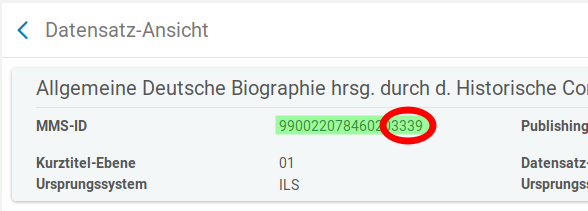
\includegraphics[width=.9\linewidth]{/home/schuhs/projects/multi-hol/doc/pic/mmsid_bib.png}
\end{center}

Diese Nummer muss mit \texttt{99} anfangen und mit \texttt{3339} aufhören. Öffnen Sie
den Texteditor -- einfach Windows-Taste drücken und "`Editor"' eingeben: 

\begin{center}
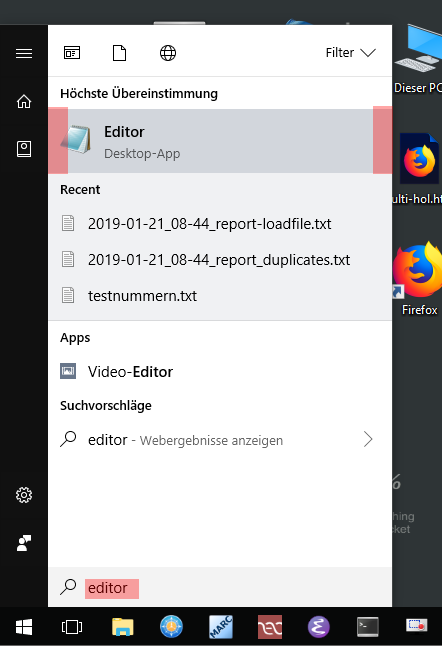
\includegraphics[width=.9\linewidth]{/home/schuhs/projects/multi-hol/doc/pic/start_edit.png}
\end{center}

Kopieren Sie die Nummer hinein.
\subsubsection{Das Ziel-Holding identifizieren/anlegen}
\label{sec:org2cf53e8}
In den allermeisten Fällen müssen Sie das Zielholding neu anlegen. Das
geht aber recht schnell:

\begin{enumerate}
\item Suchen Sie ein beliebiges Holding am gleichen Standort, mit der
Grundsignatur, die Sie brauchen und öffnen Sie dieses im Metadateneditor
zum bearbeiten
\item Klicken Sie auf [Datei -> Duplizieren]
\item Im duplizierten Holding (erkennbar am ausgegrauten Symbol) löschen Sie
den hinteren Teil der Signatur, sodass nur die Grundsignatur übrig bleibt:

\begin{center}
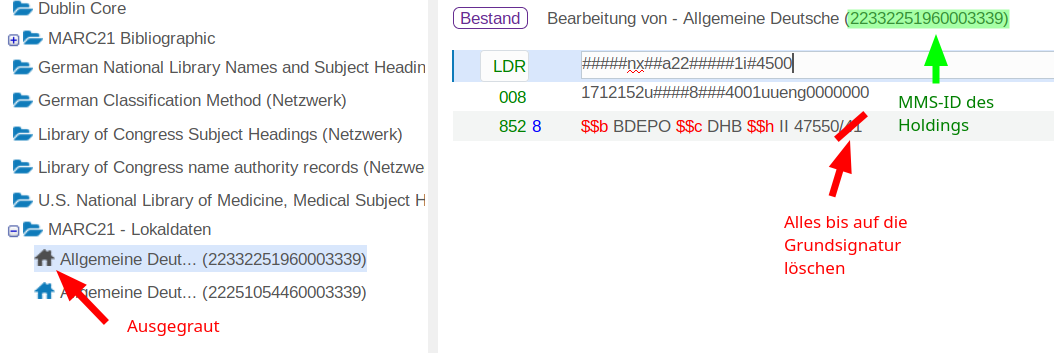
\includegraphics[width=.9\linewidth]{/home/schuhs/projects/multi-hol/doc/pic/dupliziertes_hol.png}
\end{center}
\item Klicken sie auf \texttt{Speichern}
\item Kopieren Sie die MMS-ID des Holdings (siehe den grünen Pfeil im Bild bei
Punkt 3) auch in den Editor. Die MMS-ID eines Holdings beginnt immer
mit \texttt{22} und endet mit \texttt{3339}. Im Bild sehen Sie das Editorfenster mit
der MMS-ID des Bibsatzes in der ersten und der des Holdings in der
zweiten Zeile.

\begin{center}
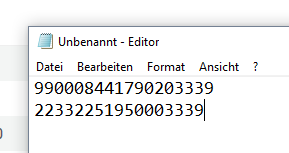
\includegraphics[width=.9\linewidth]{/home/schuhs/projects/multi-hol/doc/pic/mmsid_editor.png}
\end{center}
\end{enumerate}
\subsubsection{Das Programm ausführen}
\label{sec:orgaa2b7b1}
Jetzt, wo Sie das Zielholding angelegt haben und die MMS-IDs vom
bibliografischen Datensatz und vom Holding in den Editor kopiert haben,
können Sie das Programm ausführen. Wo es genau liegt, haben Sie
normalerweise bei der Einschulung erfahren, wahrscheinlich haben Sie auch
eine Verknüpfung auf Ihrem Desktop. Machen Sie einen Doppelklick auf das
Programm und nach ein paar Sekunden kommt ein Eingabefenster:

\begin{center}
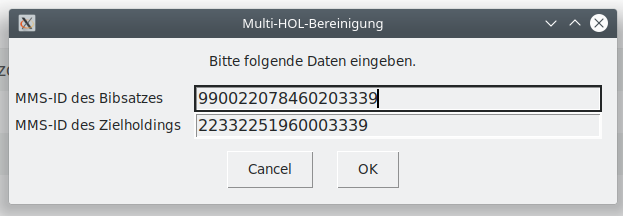
\includegraphics[width=.9\linewidth]{/home/schuhs/projects/multi-hol/doc/pic/eingabefenster.png}
\end{center}

Fügen Sie die jeweiligen Nummern in die entsprechenden Felder ein und
klicken Sie auf "`OK"'.

Im schwarzen Fenster das sich auch mit dem Programm geöffnet hat, sehen
Sie den Fortschritt der des Programms. Wenn es fertig ist, sehen Sie die
Zeilen

\begin{center}
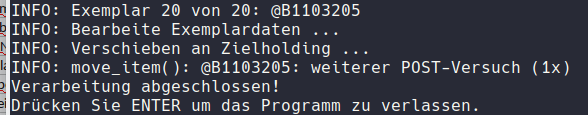
\includegraphics[width=.9\linewidth]{/home/schuhs/projects/multi-hol/doc/pic/verarbeitung_abgeschlossen.png}
\end{center}

Wenn Sie \texttt{ENTER} drücken, schließt sich das Fenster und das Progamm ist beendet.
\subsubsection{Die Zusammenfassende Bestandsangabe, etc. in Zielholding eintragen}
\label{sec:orga2c8de8}
Nach Ausführung des Programms sollte es am Datensatz für Ihre Signatur nur
noch ein Holding geben, an dem alle Exemplare hängen. Überprüfen Sie, was
da ist und machen Sie eine entsprechende zusammenfassende Bestandsangabe
im Holding.

Es ist empfehlenswert, diesen Schritt am Schluss zu machen, weil es sein
kann, dass die Bearbeitung mit weiteren Grundsignaturen ("`N.F."', etc.;
siehe \ref{sec:orgf0297ec})
wiederholt werden muss. Erst wenn alle Exemplare richtig hängen, lassen
sich die Angaben in den Holdings korrekt machen.
\subsection{Spezialfälle}
\label{sec:org1008a84}
\subsubsection{Mehrere Grundsignaturen an einem bibliografischen Datensatz}
\label{sec:orgf0297ec}
Manchmal ist es notwendig, die Exemplare an einem bibliografischen
Datensatz auf mehrere Holdings aufzuteilen. Das kommt dann vor, wenn es
mehrere Zählfolgen gibt. Jede dieser Zählfolgen hatte eine eigene \hyperref[sec:org9ca78c5]{Grundsignatur}, 
für die jeweils ein eigenes Holding angelegt werden muss.

Wenn wir uns das Beispiel von \ref{sec:org6f9a054} noch einmal ansehen,
bemerken wir, dass die Signaturen \texttt{II 47550/3} und \texttt{II 47550/N.F.2} beide
dem gleichen Zielholding zugeordnet werden. Nachdem der Anfang der
Signatur übereinstimmt, lässt sich das nicht verhindern. Im Endeffekt
funktioniert das Ganze aber trotzdem, wenn wir die Signaturen in der richtigen
Reihenfolge, nämlich beginnend mit der kürzesten Signatur, abarbeiten.

Würden wir diese Reihenfolge nicht einhalten, d. h. z. B. zuerst \texttt{II
      47550/N.F.} und erst dann \texttt{II 47550} bearbeiten, würden beim zweiten Lauf
die Exemplare alle von \texttt{II 47550/N.F.} wegwandern und sich an \texttt{II 47550}
hängen (weil ihre Signatur ja auch mit \texttt{II 47550} beginnt). Umgekehrt
passiert das nicht, weil z. B. \texttt{II 47550/23} ja nicht mit \texttt{II 47550/N.F.}
anfängt.

Das kling komplizierter, als es in der Praxis ist:

\begin{enumerate}
\item Zuerst das Zielholding für die \emph{kürzeste} Signatur anlegen und das
Programm ausführen. Damit hängen sich \emph{alle} Exemplare an dieses
Holding.
\item Danach das Zielholding für die nächste Signatur (z. B. \texttt{II 47550/N.F.})
anlegen und das Programm ausführen. Damit wandern die Exemplare der
Neuen Folge vom ersten Zielholding an das richtige. An diesem Punkt ist
die Reihenfolge nicht mehr wichtig, d. h. es ist egal ob man jetzt mit
der neuen Folge oder der 3. Serie weitermacht.
\item Diesen Vorgang mit allen notwendigen Grundsignaturen wiederholen, bis alle
Exemplare beim richtigen Holding sind.
\end{enumerate}
\begin{enumerate}
\item Ein Beispiel für mehrere Signaturen
\label{sec:orgcb3a6a4}
Hier ein Screenshot der Holdings-Liste vor der Bearbeitung, an jedem HOL
gibt es genau ein Exemplar:

\begin{center}
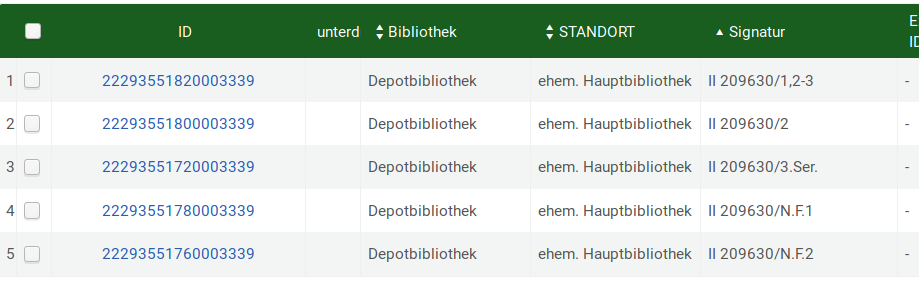
\includegraphics[width=.9\linewidth]{/home/schuhs/projects/multi-hol/doc/pic/holdings_vorher.png}
\end{center}

Nachdem wir ein Holding für \texttt{II 209630} angelegt und unser Programm haben
laufen lassen, gibt es nur noch ein Holding (dafür mit 5 Exemplaren):
\begin{center}
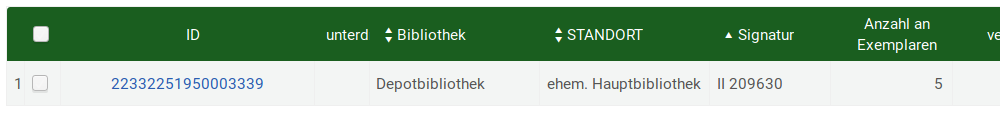
\includegraphics[width=.9\linewidth]{/home/schuhs/projects/multi-hol/doc/pic/holding_nachher.png}
\end{center}

Wenn wir die Exemplare dieses Holdings anzeigen lassen, sehen wir in der
alternativen Signatur die einzelnen Signaturen für die Exmplare. Auch die
neue Folge und die 3. Serie sind hier vertreten:

\begin{center}
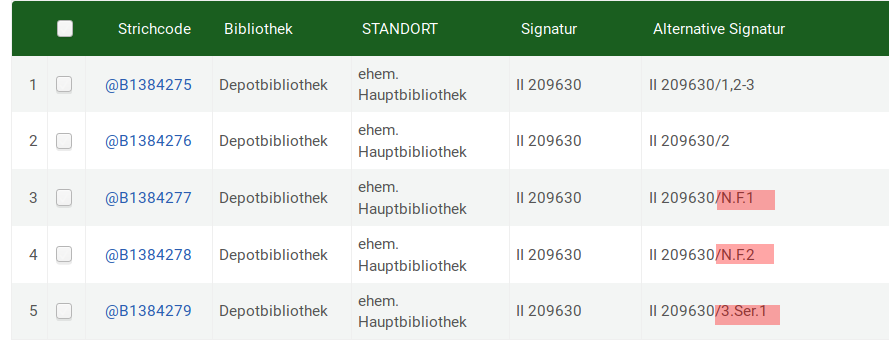
\includegraphics[width=.9\linewidth]{/home/schuhs/projects/multi-hol/doc/pic/exemplare_nachher1.png}
\end{center}

Also legen wir ein weiteres Holding mit der Signatur \texttt{II 209630/N.F.} an
und führen das Programm noch einmal aus. Wieder die gleiche MMS-ID für den
Bibsatz, aber die MMS-ID für das gerade angelegte neue Holding. Danach
gibt es zwei Holdings:

\begin{center}
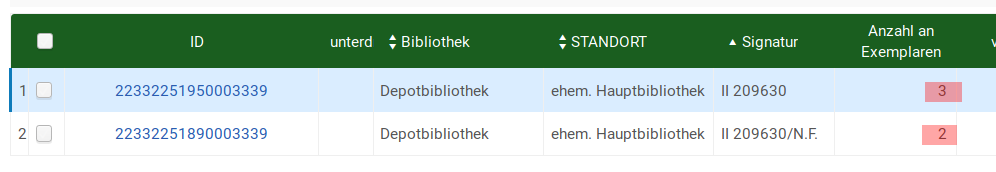
\includegraphics[width=.9\linewidth]{/home/schuhs/projects/multi-hol/doc/pic/holdings_nachher2.png}
\end{center}

Wir sehen, dass bei \texttt{II 209630} nur noch drei Exemplare sind, die anderen
beiden sind zu \texttt{II 209630/N.F.} gewandert. Nun fehlt uns noch das eine
Exemplar für die 3. Serie. Also legen wir noch ein Holding mit \texttt{II
        209630/3.Ser.} an und lassen das Programm noch einmal laufen. Dann gibt es
drei Holdings:

\begin{center}
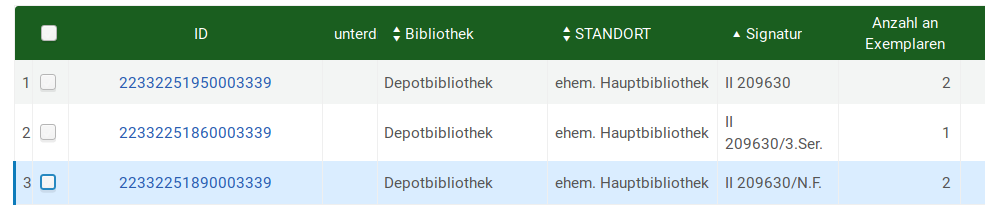
\includegraphics[width=.9\linewidth]{/home/schuhs/projects/multi-hol/doc/pic/holdings_nachher3.png}
\end{center}

Wenn wir alle Exemplare anzeigen und dort die Signatur und die alternative
Signatur ansehen, sehen wir, dass jetzt alles richtig hängt:

\begin{center}
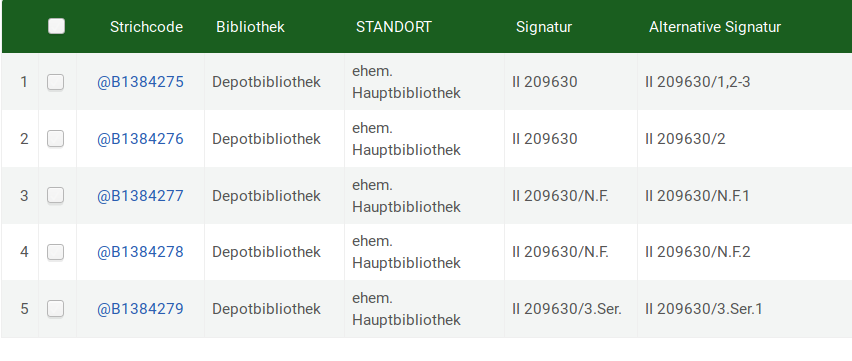
\includegraphics[width=.9\linewidth]{/home/schuhs/projects/multi-hol/doc/pic/exemplare_nachher2.png}
\end{center}

Nun können wir die restlichen Daten in den Holdings nachtragen:

Bei \texttt{II 209630}:
\begin{center}
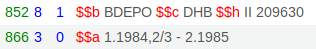
\includegraphics[width=.9\linewidth]{/home/schuhs/projects/multi-hol/doc/pic/bestand1.png}
\end{center}

Bei \texttt{II 209630/N.F.}:
\begin{center}
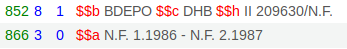
\includegraphics[width=.9\linewidth]{/home/schuhs/projects/multi-hol/doc/pic/bestand2.png}
\end{center}

Bei \texttt{II 209630/3.Ser.}:
\begin{center}
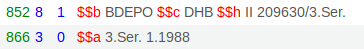
\includegraphics[width=.9\linewidth]{/home/schuhs/projects/multi-hol/doc/pic/bestand3.png}
\end{center}
\end{enumerate}
\subsubsection{Fehlermeldungen}
\label{sec:org7455f5e}
Wenn alles reibungslos funktioniert sehen sie in dem Terminalfenster, das
sich mit dem Programm öffnet, diverse Informationen vorbeiziehen. Was
diese genau bedeuten, muss Sie nicht weiter interessieren. Sie sehen das
nur, damit Sie wissen, dass das Programm etwas tut -- es kann nämlich
recht lange dauern, wenn viele Exemplare umgehängt werden. Führen Sie das
Programm also lieber nicht aus, kurz bevor Sie nachhause gehen wollen. ;-)

Normalerweise beginnt jede einzelne Zeile mit \texttt{INFO:}. Wenn das der Fall
ist, ist alles ok. Es kann aber auch sein, dass einmal eine Zeile mit
\texttt{ERROR:} beginnt. Dann hat etwas nicht funktioniert. Üblicherweise
passiert das, wenn ein Exmplar entlehnt ist, oder eine Bestellung mit dem
Exemplar oder dem Holding verbunden ist.

Das ist in den meisten Fällen kein Grund zur Besorgnis: Das Programm läuft
weiter und lässt das betroffene Holding samt Item in Ruhe. Allerdings
müssen Sie diese dann manuell bereinigen. Das heißt, wenn eine Bestellung
damit verbunden ist, diese entsprechend bearbeiten, nämlich mit dem
Zielholding verbinden. Wenn das Exemplar entlehnt ist, müssen Sie eh
warten, bis es zurück ist und können es dann umhängen.

Hier zwei Beispiele für typische Fehlermeldungen:

\phantomsection
\label{org6ba1dfd}
\begin{verbatim}
ERROR - move_item(): löschen fehlgeschlagen bei @B1103200. {"errorsExist":true,
"errorList":{"error":[{"errorCode":"401849","errorMessage":"Item delete errors:
There is a PO line POL-13073 linked to this item @B1103200. Please handle the 
order (using the PO line pages) before withdrawing this item / these items. \n",
"trackingId":"E01-2101110719-OYNS8-AWAE1622782160"}]},"result":null}
\end{verbatim}
\end{document}